\section{Results and discussion}\label{results}
This section presents the results of the Austrian case study. \added{Particularly, the mix of heat sources/generation technologies and related district heating networks in the four different scenarios (section \ref{res:1}) are presented.} \deleted{Four different storylines are investigated, covering a wide range of possible future developments of the Austrian energy system in the context of European deep decarbonization.} \deleted{Section \ref{res:1} shows the heat generation mix supplying the heat demand (residential and commercial) at the country level.} Section \ref{res:2} \replaced{presents the heat generation mix on the country, sub-regional and community levels.}{the heat generation mix obtained on a more granular geographical scale, at sub-regional and community levels.} Potentials of \replaced{district heating networks}{a centralized heat network´} are presented further in section \ref{res:3}. Section \ref{res:4} shows \replaced{district heating networks}{the centralized heat networks} at the community level. \replaced{Furthermore}{Finally}, section \ref{res:5} compares the projected \replaced{district heating}{centralized heat} networks in 2050 with today's networks, based on heat density. \added{Finally, section \ref{sens:hp} presents a sensitivity analysis of heat density on large-scale heat pump (air) generation feeding into district heating networks.}

\newcolumntype{R}[2]{%
	>{\adjustbox{angle=#1,lap=\width-(#2)}\bgroup}%
	l%
	<{\egroup}%
}
\newcommand*\rot{\multicolumn{1}{R{90}{-0.5em}}}
\newcommand*\rots{\multicolumn{1}{R{90}{1em}}}
\definecolor{Gray}{gray}{0.85}

\subsection{Heat technology generation in 2050 on different spatial granularities}\label{res:2}
Figure \ref{fig:res1} shows the heat generation per technology/source on different spatial granularities: the country (NUTS0), sub-region (NUTS3), and community (LAU) levels (from left to right). The level of spatial details increases from the left to the right. In the middle, the residential and commercial heat supply in representative rural and urban sub-regions, respectively, is presented. The rural sub-region Mostviertel-Eisenwurzen (NUTS3 code AT121) shows high shares of heat pump (air \added{ and }sourced) \added{generation}\deleted{ and small-scale heat storage systems}. Furthermore, \replaced{biomass and direct electric}{synthetic gas and direct electric} heating systems supply heat demands. The urban sub-region \replaced{Rheintal-Bodenseegebiet (AT342)}{\textit{South Viennese environs} (AT127)} is supplied by synthetic gas and waste in addition to the heat sources already mentioned. Throughout the pie charts within the figure, shares of heat generation used in district heating networks are indicated by blue edges. On the extreme right, an example of district heating at the community level in Rheintal-Bodenseegebiet (AT342) for the four scenarios is presented by highlighting the supply areas. The largest supply areas of district heating are in the \textit{Gradual Development} and \textit{Techno-Friendly} scenarios. Note that the obtained district heating supply areas not necessarily are interconnected. Exemplarily, two separated communities are supplied by district heating in the \textit{Directed Transition} scenario.

\begin{sidewaysfigure}
	\centering
	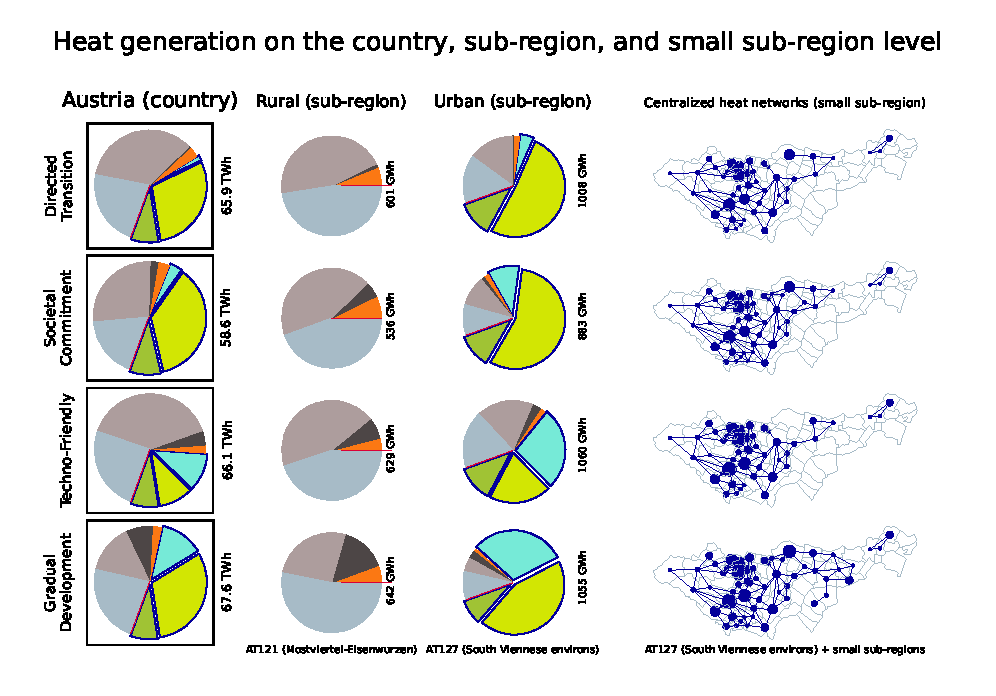
\includegraphics[width=1\linewidth]{figures/4_Results/Fig_Matrix-plot/Spatial_results.eps}
	\caption{Heat technology generation on different spatial granularity levels in the different scenarios supplying the residential and commercial heat demand. left: on the country level. middle: comparison of a rural and urban sub-region. right: \replaced{district}{centralized} heat\added{ing} \deleted{network}\replaced{at the community level}{topology (size of the points represent the amount of heat demand supplied by the network)}}
	\label{fig:res1}
\end{sidewaysfigure}

\subsection{Sub-regions in Austria 2050 with potentials for district heating}\label{res:3}
\added{Figure \ref{fig:res2} presents heat demand supplied by district heating in Austria in 2050 on the NUTS3 level. Heat demands in the four sub-regions Vienna (AT130), Graz (AT221), Linz-Wels (AT312), and Rheintal-Bodenseegebiet (AT342) are covered by district heating in each scenario. The remaining sub-regions ($31$ out of $35$) are supplied exclusively by on-site heat generation technologies/sources. However, the amount of district heating in the sub-regions varies significantly between the scenarios (see also the bottom column in Table \ref{tab:comparison}). For each sub-region, the highest amount of district heating is in the \textit{Gradual Development} scenario. Table \ref{tab:3} presents the quantitative results of district heating and on-site heat supply in the four sub-regions and scenarios. The share of district heating in the \textit{Directed Transition} scenario is between 15\% and 38\% in the sub-regions. Against this, the \textit{Gradual Development} scenario has shares between 86\% and 99\%.}

\begin{table} \centering
	\resizebox{0.9\textwidth}{!}{% use resizebox with textwidth
		\renewcommand{\arraystretch}{1.1}
		\begin{tabular}{cccccc}
			\toprule 
			&& \multicolumn{2}{c}{in TWh} & in \%\\\cmidrule(lr){3-4}\cmidrule(lr){5-5}
			Sub-region & Scenario&District heating (DH) & On-site & Share of DH\\\hline
			 \parbox[t]{15mm}{\multirow{4}{*}{\rotatebox[origin=c]{90}{\parbox{2cm}{\centering Vienna\\(AT130)}}}} & Directed Transition & 4.22 & 6.76 & 38\\
			 & Societal Commitment & 5.70 &  4.62 & 55\\
			 & Techno-Friendly & 10.11 &  0.58 & 95\\
			 & Gradual Development & 11.12 &  0.07 & 99\\\hline
			  \parbox[t]{15mm}{\multirow{4}{*}{\rotatebox[origin=c]{90}{\parbox{2cm}{\centering Graz\\(AT221)}}}} & Directed Transition & 0.38 & 2.17 & 15\\
			 & Societal Commitment & 0.60 &  1.80 & 25\\
			 & Techno-Friendly & 1.34 & 1.14 & 54\\
			 & Gradual Development & 2.25 & 0.35 & 87\\\hline
			 \parbox[t]{15mm}{\multirow{4}{*}{\rotatebox[origin=c]{90}{\parbox{2cm}{\centering Linz-Wels\\(AT312)}}}} & Directed Transition & 0.51 & 2.91 & 15\\
			 & Societal Commitment & 0.80 & 2.42 & 25\\
			 & Techno-Friendly & 1.80 & 1.53 & 55\\
			 & Gradual Development & 3.03 & 0.46 & 87\\\hline
			 \parbox[t]{15mm}{\multirow{4}{*}{\rotatebox[origin=c]{90}{\parbox{2cm}{\centering Rheintal-Bodensee\\(AT342)}}}} & Directed Transition & 0.27 & 1.54 & 15\\
			 & Societal Commitment & 0.42 & 1.28 & 25\\
			 & Techno-Friendly & 0.96 & 0.81 & 54\\
			 & Gradual Development & 1.60 & 0.25 & 86\\
			\bottomrule
	\end{tabular}}
	\caption{District heating and on-site heat supply in the four Austrian sub-regions with district heating networks in 2050.}
	\label{tab:3}
\end{table}

\begin{sidewaysfigure}
	\centering
	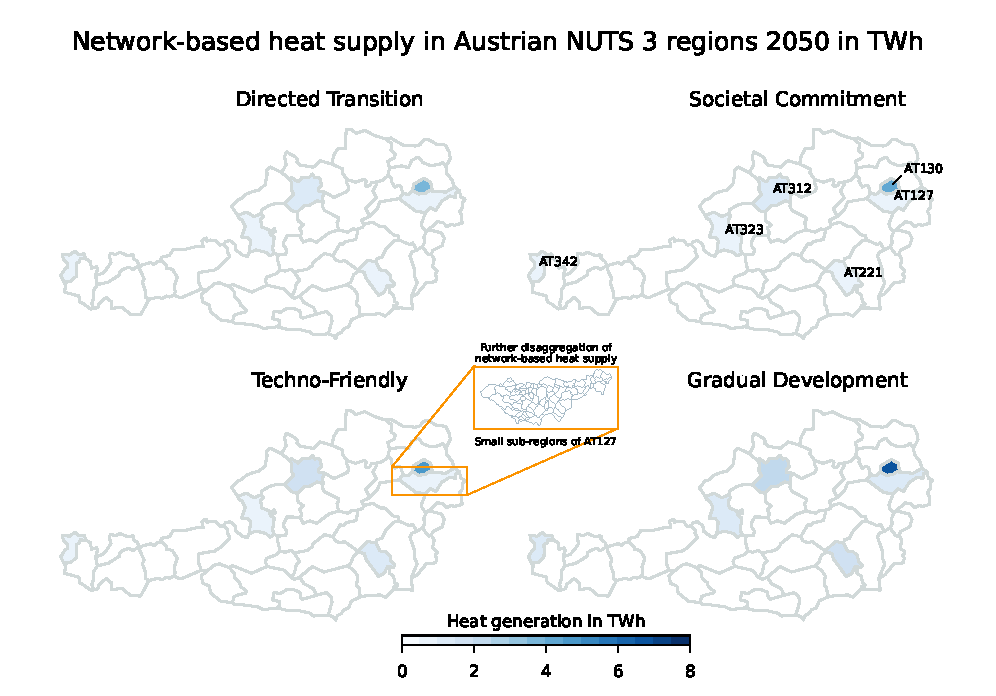
\includegraphics[width=1\linewidth]{figures/4_Results/Fig-Heatmap/Heatmap.eps}
	\caption{Heat demand supplied by district heating in Austria 2050. White sub-regions are supplied exclusively by on-site heat generation technologies/sources.}
	\label{fig:res2}
\end{sidewaysfigure}

\subsection{\replaced{District}{Centralized} heat\added{ing} network topology at the community level}\label{res:4}
This section presents the \replaced{district}{centralized} heat\added{ing} network topology of the sub-region \replaced{\textit{Linz-Wels} (AT312)}{\textit{South Viennese environs} (AT127)} and all included communities \added{in the \textit{Directed Transition} scenario}. \deleted{In Figure \ref{fig:res2}, this particular sub-region is marked by the orange box.} Figure \ref{fig:res3} \added{(the two subfigures at top)} shows the projected \replaced{district heating supply area}{centralized heat network topology}. In particular, the network topology is presented for the initial condition (as a result of the sequential downscaling, $i=1$) and the final condition of the network \added{(as a result of the iterative downscaling}, $i=65$). The distribution of the benchmark indicator values of the \replaced{district}{centralized} heat\added{ing} network depending on the number of iterations is presented in the middle. Particularly, the \replaced{median}{mean value} is marked in orange. The supply area decreases with an increasing number of iterations. In the community analyzed here, the termination criterion of the algorithm is reached when \replaced{10}{25} communities are connected (starting from \replaced{74}{75} in the initial condition). \added{The population of connected communities decreases by 40\%, starting from a population of 663,000 in the initial condition. After the final iteration} ($i=65$), \added{the termination criterion is reached, and the population of connected communities is 397,000.}

\begin{sidewaysfigure}
	\centering
	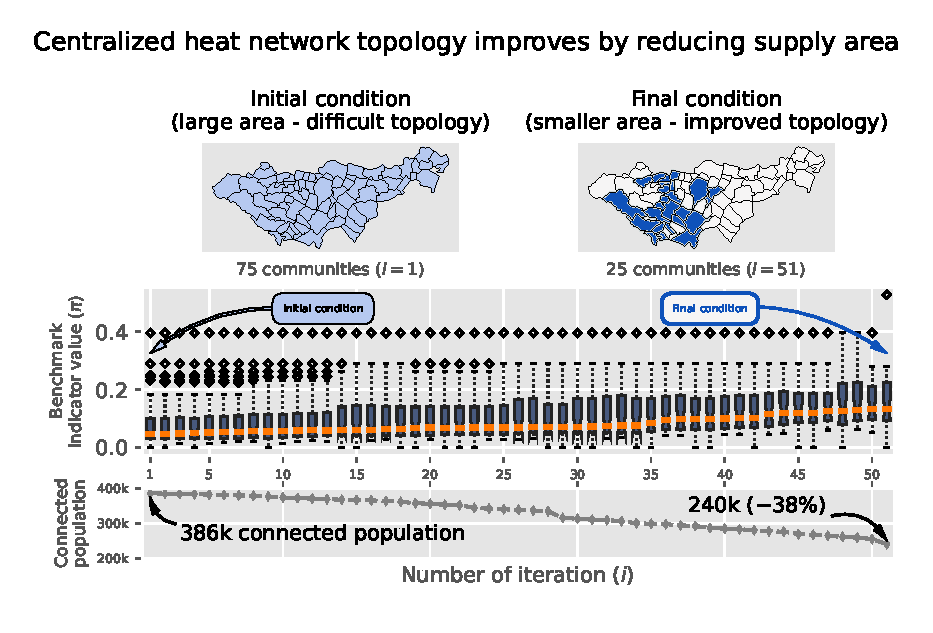
\includegraphics[width=1\linewidth]{figures/4_Results/Fig_Boxplot/ext_boxplot.eps}
	\caption{\replaced{District}{Centralized} heat\added{ing} network topology \replaced{in Linz-Wels (AT312) in the \textit{Directed Transition} scenario}{in the initial and final condition}. The boxplot (middle) indicates the improved network topology by \deleted{an} increasing benchmark indicator \replaced{values}{mean value (orange line)}. In the final condition \added{10 communities; i=65}, the \replaced{population of connected communities}{connected population} declines by \SI{-40}{\%} compared to the initial condition (74 communities; i=1).}
	\label{fig:res3}
\end{sidewaysfigure}

\subsection{Comparison of 2050's and today's \replaced{district}{centralized} heat\added{ing} networks using heat density as a criteria}\label{res:5}
In the following, the \replaced{district}{centralized} heat\added{ing} network in \replaced{Linz-Wels (AT312)}{\textit{Graz} (AT221)} is shown in detail. This area is selected for illustrative purpose, because it provides representative results in terms of both the applied downscaling and achievable heat density benchmarks of district heating networks. Figure \ref{fig:res5} shows the heat density of \replaced{district heating}{the centralized heat network} in the \textit{Techno-Friendly} scenario. The x-axis shows the three different downscaling techniques. The numerical numbers indicate a significant increase of the heat density by the sequential (+\SI{0.49}{GWh \per km^2}) and, in particular, the iterative downscaling (+\SI{3.21}{GWh \per km^2}). However, comparing the heat density value obtained with the heat density values of today's district heating networks reveals a significant gap (see the hatched pink bar). Here, in the \textit{Techno-Friendly} scenario, it is \SI{5.75}{GWh \per km^2}. According to references from the practice (\deleted{see, e.g., in}\url{http://www.austrian-heatmap.gv.at/ergebnisse/}), the \added{threshold} heat density of today's networks is assumed to be \SI{10}{\frac{GWh}{km^2}} with a connection rate of \SI{90}{\%}.

\begin{figure}[h]
	\centering
	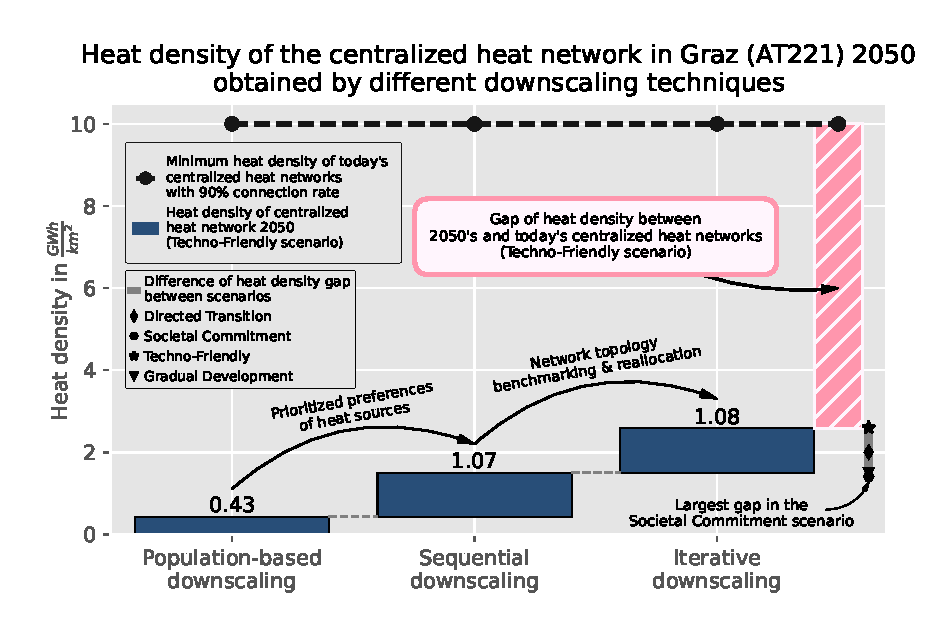
\includegraphics[width=0.9\linewidth]{figures/4_Results/Fig_Heat-density/HD_cleaned1.eps}
	\caption{Heat density of the \replaced{district}{centralized} heat\added{ing} \deleted{network} in \replaced{Linz-Wels (AT312)}{\textit{Graz} (AT221)} 2050 in the \textit{Techno-Friendly} scenario. The gap of heat density between 2050s and today (black dashed line) is marked by the pink bar.}
	\label{fig:res5}
\end{figure}

\subsection{Allocation of heat pump (air) generation into district heating}\label{sens:hp}
\added{Building upon Figure \ref{fig:res5}, the following sensitivity analysis examines the heat density for each network and scenario under an increasing allocation of heat pump (air) generation into district heating. In particular, it investigates how the heat density (and its gap) change under an increasing amount of district heating (i.e., heat generation used in district heating). The total heat pump (air) generation of the cost-effective GENeSYS-MOD results is divided into small- and large-scale heat pump (air) generation. Here, large-scale heat pump (air) generation is used in district heating. Figure \ref{fig:sens} in} \ref{Appendix:D} \added{shows the heat density of the the district heating network in Graz (AT221) in the \textit{Directed Transition} scenario. The figure illustrates the influence of the increasing allocation of large-scale heat pump (air) generation into district heating on the heat density. For example, the maximum heat density is reached at a share of two-thirds of large-scale heat pump (air) generation.}\vspace{0.3cm}

\begin{figure}[h]
	\centering
	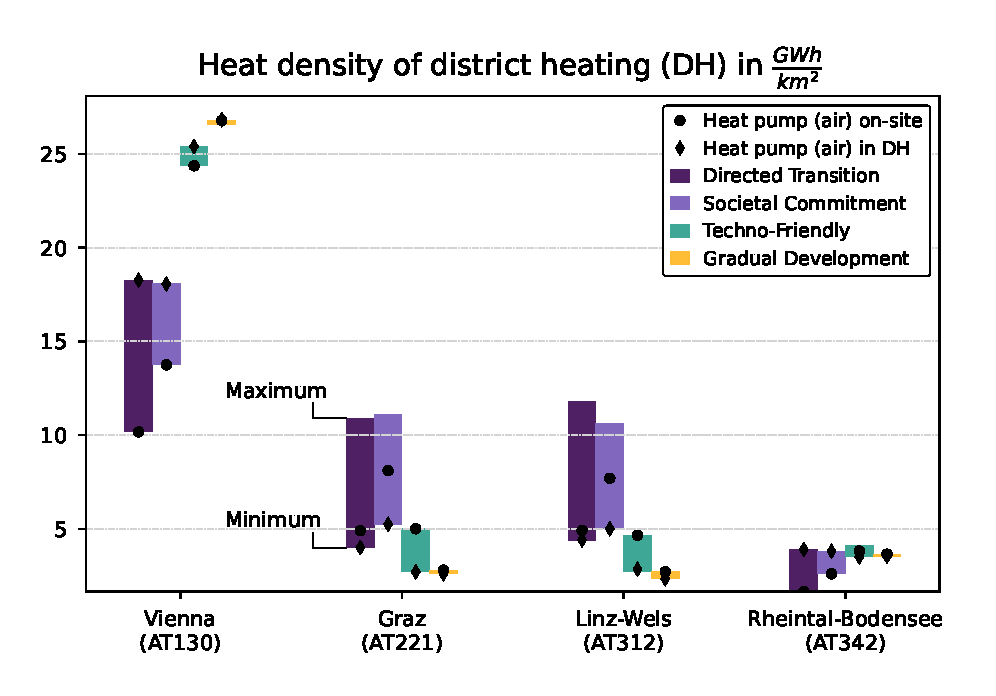
\includegraphics[width=1\linewidth]{figures/4_Results/Max_Heatdensity/4x4.eps}
	\caption{\added{Heat density of district heating networks in the four sub-regions and scenarios in 2050 for varying allocation of heat pump (air) generation between large- and small-scale. The optimal allocation of large-scale heat pump (air) generation results in some cases in heat densities above the threshold required for economic viability in current systems (e.g., Graz (AT221) in the \textit{Directed Transition} scenario).}}
	\label{fig:max_heat_densities}
\end{figure}

\added{Figure \ref{fig:max_heat_densities} shows the heat density in the four sub-regions and scenarios. The range of heat density resulting from different shares of large-scale heat pump (air) generation is presented. The two extreme points that only small-scale or large-scale heat pump (air) units are used in the sub-regions are marked by the black circle (i.e., heat pump (air) on-site) and diamond (i.e., heat pump (air) in district heating). Particularly, the heat density in the \textit{Directed Transition} and \textit{Societal Commitment} scenario increases significantly compared with on-site heat pump (air) generation only (e.g., Graz (AT221) and Linz-Wels (AT312)). In Vienna (AT130), the heat density remains almost the same in the \textit{Techno-Friendly} and \textit{Gradual Development} scenario. At the same time, the heat density there increases and reaches} \SI{18}{GWh \per km^2} \added{in the \textit{Directed Transition} and \textit{Societal Commitment} scenario. In Rheintal-Bodensee (AT342), the heat densities are relatively low compared to the others, independently of the allocation of large-scale heat pump (air) generation to district heating.}

